\documentclass[a4paper]{article}
\usepackage{amsmath}
\usepackage{graphicx}
\usepackage{longtable}
\usepackage{makecell}
\usepackage[most]{tcolorbox}
\usepackage{listings}
\usepackage{csquotes}

\title{DRLND Collaboration and Competition- Report}
\date{2018-12-31}
\author{Matthias Schinacher matthias.schinacher@googlemail.com}

\begin{document}

\maketitle
\tableofcontents
\newpage

\section{Intro}
The project is a homework assignment for Udacity's \textbf{Deep Reinforcement Learning Nano Degree}.
The project ist the third one called \textit{Collaboration and Competition}.
\\
The project environment is a course provided version of the Unity \enquote{Tennis}
environment of the ML- agents Unity has on the respective github- page.
The environment has two \enquote{agents} that play a game resembling tennis.
\\
Each agent, represented as a crude form of tennis racket, has 2 continuous-value actions;
move towards/ away from the net and move up/ down. If an agent lets the ball
reach it's side of the court or shoots the ball outside the court, a negative
\enquote{reward} of -0.01 is earned and if the agent manages to play the ball
across the net, it gets 0.1 as a reward.
\\
The goal is to get as high a reward as possible, and as there is no reward
for an agent, when the other agent fails, this means to keep the ball in play
as long as possible.
\\
For this project I chose to implement DDPG with experience replay and
a variant of priority replay in a python script to be invoked from command line.
\\
I derived the script from the one I wrote for the \enquote{Continuous Control}- project,
which itself was based partially on my script for the \enquote{Navigation}- project.
\\
The DDPG needs 4 approximations (actor, critic and the 2 target- variants of them)
that I modeled as neural networks with fully connected layers, ReLU layers,
$Tanh$- layers using PyTorch.

\section{Implementation}
\subsection{Python script}
The script is named $ms\_drlnd\_collab\_comp.py$ and must be invoked from the command
line with exactly one parameter, the name of the ".ini"- file (a.k.a. command file),
that has all the parameters.
\\
\textit{The $\delta$ of the prio-replay, upon which the priority of a transition
is based, uses the difference between the state-action value the critic
computes and the estimation of this value by the target critic using the reward
and the target critics state-action value of the subsequent state.\\
The prio-replay implementation partially follows the \enquote{PRIORITIZED EXPERIENCE REPLAY}
paper by Tom Schaul, John Quan, Ioannis Antonoglou and David Silver}

\paragraph{Parameters}
The parameters listed in the command file come in various sections. The basic format
is similar to the Windows style INI files and is the one that pythons $configparser$
module uses (as the module is used in the script).

\subparagraph{Example}
:\\
\tiny

\texttt{
{[global]} \\
runlog = test11.log \\
{[mode]} \\
train = True \\
show = False \\
{[rand]} \\
seed = 14111 \\
{[model]} \\
save\_file  = test11 \\
model\_h1   = 411 \\
model\_h2   = 277 \\
model\_c\_h1 = 409 \\
model\_c\_h2 = 279 \\
batch\_norm = False \\
{[hyperparameters]} \\
episodes          = 1500 \\
warmup\_episodes   = 50 \\
warmup\_episodes\_f = 0.4 \\
replay\_buffersize = 10000 \\
replay\_batchsize  = 384 \\
replay\_steps      = 1 \\
gamma             = 0.99 \\
learning\_rate     = 0.0001 \\
learning\_rate\_c   = 0.001 \\
optimizer\_steps   = 1 \\
tau               = 0.01 \\
max\_steps         = 850 \\
epsilon\_start     = 3.0 \\
epsilon\_delta     = 0.0035 \\
epsilon\_min       = 0.01 \\
noise\_theta       = 0.15 \\
noise\_sigma       = 0.2 \\
prio\_replay       = True \\
prio\_offset       = 0.2 \\
grad\_norm\_clip    = 5.0
}

\normalsize

\subparagraph{Description}
:\\
\small
\begin{tabular}{ |l|r|l|c| }
  \hline
  \multicolumn{4}{|c|}{Parameters} \\
  \hline
Section & Name & Description & Default \\
  \hline
\multicolumn{4}{|l|}{\textbf{global}} \\
               & runlog & name of the logfile to use & \texttt{run.log} \\
\multicolumn{4}{|l|}{\textbf{mode}} \\
               & train & whether we're in training mode & \texttt{True} \\
               & show & \makecell[tl]{flag, whether to show \\ the simulation in "human time"} & \texttt{False} \\
\multicolumn{4}{|l|}{\textbf{rand}} \\
               & seed & \makecell[tl]{seed for \\ random number generation} & \makecell[tc]{no explicit \\ random seeding performed} \\
\multicolumn{4}{|l|}{\textbf{model}} \\
               & h1 & \makecell[tl]{first size- parameter \\ for the actor- NN- model} & \texttt{311} \\
               & h2 & \makecell[tl]{second size- parameter \\ for the actor-NN- model} & \texttt{177} \\
               & c\_h1 & \makecell[tl]{first size- parameter \\ for the critic- NN- model} & \texttt{309} \\
               & c\_h2 & \makecell[tl]{second size- parameter \\ for the critic-NN- model} & \texttt{179} \\
               & load\_file & \makecell[tl]{name- fragment for the files \\ from which to load models (if any)} & None \\
               & save\_file & \makecell[tl]{name- fragment for the files \\ to save the models to} & \makecell[tc]{"\texttt{DDPG-out}" \\ if in training mode} \\
               & batch\_norm & \makecell[tl]{flag, whether batch-norm \\ layers are used \\ (currently broken)} & \texttt{False} \\
\multicolumn{4}{|l|}{\textbf{hyperparameters}} \\
               & episodes & number of episodes to run & \texttt{1000} \\
               & max\_steps & maximum number of steps in episode & \texttt{500} \\
               & warmup\_episodes & \makecell[tl]{epiosodes to run with \\ pure random sampling} & \texttt{50} \\
               & warmup\_episodes\_f & \makecell[tl]{scale factor for pure random sampling} & \texttt{0.4} \\
               & replay\_buffersize & size of the replay memory & \texttt{10000} \\
               & replay\_batchsize & \makecell[tl]{number of transitions to sample \\ per optimizing step} & \texttt{512} \\
               & replay\_steps & \makecell[tl]{simulation-steps between \\ each optimization run} & \texttt{1} \\
               & optimizer\_steps & \makecell[tl]{no. of batch optimization-steps \\ per optimization run} & \texttt{1} \\
               & learning\_rate & the learning rate for the actor & \texttt{0.0001} \\
               & learning\_rate\_c & the learning rate for the critic & \texttt{0.001} \\
               & gamma & $\gamma$ & \texttt{0.99} \\
               & tau & $\tau$ (soft target update) & \texttt{0.01} \\
               & grad\_norm\_clip & \makecell[tl]{threshold for grad-norm clipping; \\ negative means no clipping} & \texttt{-1.0} \\
\multicolumn{4}{|c|}{\textit{replay prioritization}} \\
               & prio\_replay & flag, whether to use prio- replay & \texttt{True} \\
               & replay\_offset & \makecell[tl]{used to calculate priorities \\ (see details for more info)} & \texttt{0.2} \\
\multicolumn{4}{|c|}{\textit{sample action noise}} \\
               & epsilon\_start & start value for $\epsilon$ & \texttt{2.5} \\
               & epsilon\_delta & \makecell[tl]{value to subtract from $\epsilon$ \\ for each optimization step} & \texttt{0.001} \\
               & epsilon\_min & minimum/ final value for $\epsilon$ & \texttt{0.02} \\
               & noise\_theta & $\theta$ for noise process & \texttt{0.15} \\
               & noise\_sigma & $\sigma$ for noise process & \texttt{0.2} \\
%               &  &  & \texttt{} \\
\hline
\end{tabular}
\normalsize

\begin{itemize}
\item the $train$- parameter of the script determines, if the algorithm will be learning
from new transitions.
\item though the script will try to honor $batch\_norm$, the current implementation contains
a bug, so that this feature is not usable currently!
\end{itemize}

\subsection{Dependencies}
The script has runtime dependencies; these are the ones as described in the
project instructions; I will therefore refrain from detailing the dependencies \textit{here}.

\subsection{Details/ algorithm}
The algorithm implemented is basically Deep Deterministic Policy Gradient (DDPG).
\\
The replay memory-buffer is implemented as a simple list with a specified capacity (\textit{replay\_buffersize}),
where the oldest entry is overwritten by the newest entry, if the capacity is already
fully used.
\\
The script uses a specified number (\textit{replay\_batchsize}) of transitions
to perform the optimization step; how often the optimization step is performed
is determined by \textit{replay\_steps}, that is once every \textit{replay\_steps}
simulation-steps the optimization is performed, and \textit{optimizer\_steps}
controls how many batches/ optimization steps are performed in sequence then.
Also a noise- adjustment of the sampled actions is used.

\paragraph{Prio- replay}
Also the script implements priority replay partially following \enquote{PRIORITIZED EXPERIENCE REPLAY}
paper by Tom Schaul, John Quan, Ioannis Antonoglou and David Silver.
By using the \textit{prio\_replay} flag/ parameter, replay prioritization can be
turned on/off per simulation run.\\
The priorities computed for the actually sampled transitions to update the
replay- priorities in the replay buffer are not simply the $\delta$'s for
the transitions, but are computed using the \texttt{replay\_offset}- parameter
to be $(replay\_offset + \delta)^2$.

\paragraph{Warmup episodes}
The script/ program computes the action values to be used randomly for
a number episodes (\textit{warmup\_episodes}), before the actual actor- model
is used. The values are sampled from the standard normal distribution and
mupltiplied by the factor \textit{warmup\_episodes\_f} before they are clipped
to the range -1 to 1.

\paragraph{Sampling noise}
When not in warmup, the action values are computed using the actor model,
to which a noise (times $\epsilon$) is added. The noise is computed by
$noise = noise -\theta noise + \sigma random\_number$. This noise is
initialized with zero and the \textit{random\_number} is taken from the
usual uniform distribution between 0 and 1.
\\
As the $\epsilon$ factor decreases the actual noise applied decreases also.

\paragraph{Neural Network layout}
The approximation functions for the actor and critic (the \textit{normal}
and the target variants) are implemented as neural networks using PyTorch.
\\
Each uses 3 linear layers with ReLU- layers after the first and second linear
layers. The actor model has a final $tanh()$- layer (the critic does not).
The critic inputs the only the state to the first layers and mixes the action-
input after the first ReLU by concatinating it to the ReLU layers output
(before it goes intu the second linear layer).
\\
\textbf{Note:} the script actually has an option/ a flag that would allow for
an optional batch-norm layer before the first linear layer (actor and critic),
but the implementation seems to have a bug currently (I'm planning to fix this
at some point), so the batch-norm thingy is not usable in the moment. 

\begin{tabular}{ |c|c| }
  \hline
  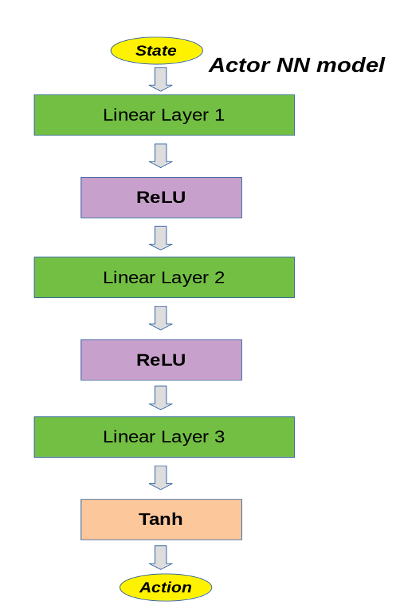
\includegraphics[scale=0.3]{ActorPic.png} & 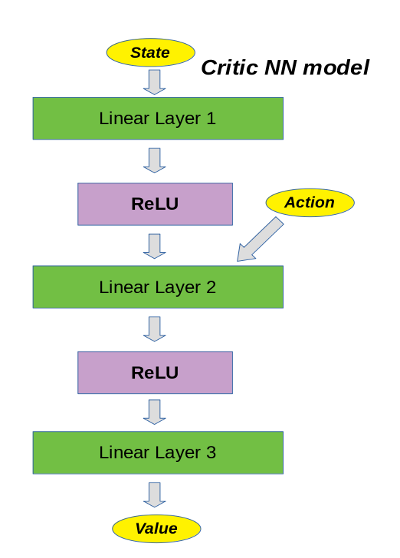
\includegraphics[scale=0.3]{CriticPic.png} \\
  \hline
\end{tabular}

\textbf{Note:} with 3 linear layers each and fixed sizes for the input
(by the unchangable values for state size and action size) as well as output
(action size and 1, cause the critic must yield a value), there are 2
choosable sizes for the actor and critic each (hence the parameters).

\paragraph{Neural Network use by the algorithm}
Though we have 2 agents in the simulation, the 4 networks (actor, critic,
target-actor and target critic) represent \textbf{one set of DDPG- networks}
which \textbf{both agents} use; but the state and action vectors fed to the
networks are technically \textbf{not} joined vectors but the \textit{local}
state and action vectors per agent.

\subparagraph{Replay buffer/ memory}
Also the replay buffer is only one replay buffer filled by both agents, thus
the algorithm registers 2 transitions per time-step, one for each agent.

\subparagraph{Learning}
Consequently the learning/ optimization of the networks uses the combined
collected transitions of the 2 agents. 

\subsection{Usage}
The script is invoked from the command line as a python script with one parameter,
a file-name from which to read all the parameters governing the algorithm.
\\
Example:\\
\texttt{python ms\_drlnd\_collab\_comp.py test05.ini}

\subsection{Loading and saving models/ pretraining}
The script is able to save the model- states of the neural networks as well as
the transitions in the replay-memory to file and/or load these from file
at the beginning of a script-run.
\\
The parameters allow for a name- fragment to be specified, from which the
actual filenames are derived. Each NN- model as well as the transitions-
replay buffer (plus priority- buffer) gets it's seperate file.
\\
The models are saved/ loaded using PyTorch's build in mechanism and the
replay- buffer file is created using pythons \textit{pickle}- module.

\small
\begin{tabular}{ |l|l| }
  \hline
  \multicolumn{2}{|c|}{file names} \\
  \hline
data & physical file name \\
  \hline
actor model & \texttt{actor\_\{fragment\}.model} \\
target actor model & \texttt{target\_actor\_\{fragment\}.model} \\
critic model & \texttt{critic\_\{fragment\}.model} \\
target critic model & \texttt{target\_critic\_\{fragment\}.model} \\
replay buffer & \texttt{transitions\_\{fragment\}.pickle} \\
  \hline
\end{tabular}
\normalsize

The saved model/ transitions allow for a subsequent script/ program- run to
pick up, where a previous run ended, effectivly using this as a pretraining.
This also allows to continue a simulation-run with adjusted algorithm parameters;
the neural net size parameters are ignored when loading aprevous model!

\subsection{Outputs}

The script prints some info to the standard output, but the actually important
output is the run-log file; it prints a (non '\#'-) textline per episode containing
the episode, the score the episode reached, the average score of the last 100
episodes (or 0, if it's an episode before the 100th), the number of steps
in the episode, the replay buffer size at the end of the episode and $\epsilon$ for the episode
separated by a blank.
The logfile can thus be read by certain programs/ tools as some sort
of time-series for the score and the average-100-last-episodes-score; one such
tool is \textbf{gnuplot}, with which I created the graphics contained in the report.

\subsection{Misc. algorithm details}
The algorithm distinguishes between \textbf{optimization run} and \textbf{optimization step}.
A optimization run occurs every \textit{replay\_steps} (when not in warmup) and
contains \textit{optimization\_steps} steps. Each such step uses a freshly sampled
batch from the replay buffer to feed it to the models as the DDPG algorithm
prescribes; 2 instances of the PyTorch Adam- optimizer are used to make a step
for actor and critic.
\\
\textbf{Note:} the target networks are soft- updated per optimization run,
and the $\epsilon$ for the action noise is also adjusted per episode.

\section{Results}
I did need quite some time experimenting with different hyper- parameters to
find a combination, that would meet the project target-score.
\\
But before I found a \textit{winning combination}, I experimented with
a different DDPG- variant. Instead of shared actor/ critic networks I used a
seperate setup per agent, where each agent had it's own set of actor/ critic-
networks (normal and target) and it's own replay buffer.
\\
Unfortunatly, I could not find a parameter combination that would result in
meaningful learning (maybe my code still has a bug I missed?) and thus I
abandoned this approach (see the script \texttt{ms\_drlnd\_collab\_comp\_sep.py})

\subsection{Results of selected simulation runs}

\paragraph{Command files/ INI- files}
Each command file (a.k.a. INI- file) represents one \textit{experiment} (program/ script- run).
See the list below for an overview of these experiments/ command files
(refer to the actual files for details of all hyperparameters).
\\

\begin{tabular}{ |l|l| }
  \hline
Filename & Description \\
  \hline
$test10.ini$ & \makecell[tl]{simulation with actual learning \\ almost reaching the 0.5 sustained score} \\
$test11.ini$ & \makecell[tl]{first simulation solving the task} \\
$test12.ini$ & \makecell[tl]{similar parameters as $test11.ini$, \\ shows very little learning } \\
$test13.ini$ & \makecell[tl]{another parameter combination, \\ again, little learning} \\
  \hline
\end{tabular}

\paragraph{Graph- plots}

\textit{(All plots are score per episode plus average score of the last 100 episodes per episode.
Constants (e.g. 0.1 or 0.5 for target score) are plotted as reference points.)}
\\
\begin{tabular}{ |c|c| }
  \hline
  \texttt{test10.ini} & \texttt{test11.ini} \\
  \hline
  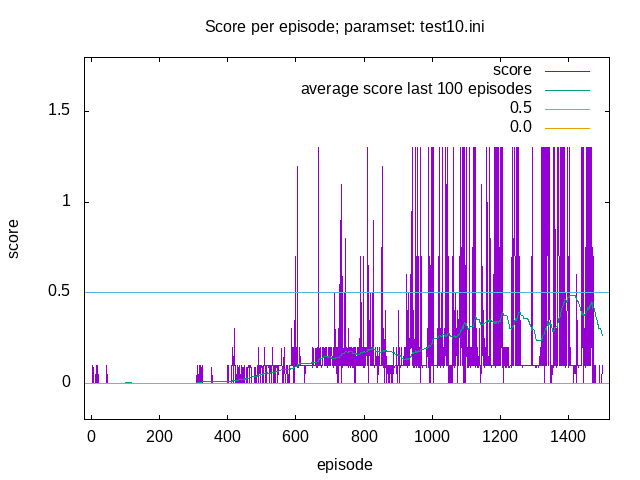
\includegraphics[scale=0.35]{test10.png} & 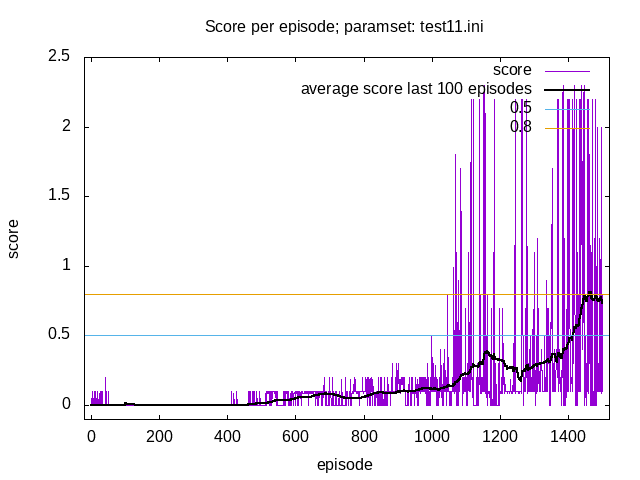
\includegraphics[scale=0.35]{test11.png} \\
  \hline
  \texttt{test12.ini} & \texttt{test13.ini} \\
  \hline
  \includegraphics[scale=0.35]{test12.png} & \includegraphics[scale=0.35]{test13.png} \\
  \hline
\end{tabular}

\subsection{Remarks/ discussion}
The \texttt{test11.ini} simulation did reach score 0.5 over the last 100 episodes
at episode 1413 and actually reached 0.8 (avrg. last 100).
\\
\texttt{test10.ini} almost reached the sought sustained score of 0.5 at episode
1412 with an average score for the last 100 episodes of 0.4875, but this decreases
the following episodes.
This \textit{failure} might in part be due to the fact, that it uses a maximum
number of steps of 500, thus cutting off the maximum score possible per episode
(\texttt{test11.ini} uses up to 850 time-steps).
\\
\texttt{test12.ini} and \texttt{test13.ini} use parameters not that vastly different
from the solving parameter-set, but show no real learning at all; I conclude
that the algorithm is quite fickle/ sensitive to the specific values of at least
some of the hyperparameters (but I did not have the time to methodically
research which parameters in which way). This is in line with the similar
experience from the other project (especially \textit{Continuous Control}).
\\
As mentioned earlier I also experimented with a setup, where each agent had it's
own set of networks and seperate replay-memory but could not get that to \textit{learn}.
I find this somehow counter- intuitive as the states and action spaces for the
2 agents are symmetric but not identical. Using one set of networks and a joined
replay buffer I was expecting to learn at least slower and with more difficulty
or maybe requiring larger networks. This seems not to be the case.

\subsection{Result models and data}
The final neural network models for the simulations (at the end of the simulation run)
can be found in the respective \texttt{*.model}- files, where they are saved
in the PyTorch specific manner; note that you need to use the \texttt{MSA} (actor) and \texttt{MSC} (critic)
classes within the script in addition to PyTorch.\\
For the \textit{solving} simulation runs, there is an additional set of
files containing not the networks states at the end of the simulation run, but
the networks at the end of the highest scoring episode \textbf{after} reaching
the sustained 0.5 score critieria (these are the \enquote{\_max.model}- files).\\
As only \texttt{test11.ini} actually solved the task, the is only one set
of these max- model files (written after episode 1417 with score 2.3)
\\
You can also kind of \enquote{print out} the models with the script
\texttt{print\_model.py}, but this will not give you all parameter values
out of the box (modify the script accordingly, if you want :-)).
\\
\subsection{ZIP files}
I zipped the resulting log-files, model files, transitions (replay buffer)- files
and INI- files in various \texttt{*.zip} archives.

\section{Possible improvements}
\subsection{Algorithm}
\paragraph{Random sampling/ noise}
The implementation uses a random-noise source to tweak the actions, that the
actor model computes for a state. Since the setup is the same as for the
previous project (\textit{Continuous Control}), the same possible modifications
apply here:
\begin{itemize}
\item applying noise to the state (input) instead of the computed actions (output)
\item currently the 2 action dimensions are supplied with noise at each step;
this could be altered by randomly choosing not to apply noise per step or
applying noise not to both actions; a variety of schemes are possible here.
\end{itemize}

\subparagraph{Tweaking $\epsilon$- decay}
Again, as with the previous projects, the $\epsilon$- decay for the noise
was rather simple, a start value, a minimum value and a delta to subtract per episode,
resulting in a linear decrease.
\\
Different to the last project, my intuition here is, that the final
$\epsilon$ value is important, but it seems to me the actual decay- scheme
not so much (but I did not really research this).\\
Nevertheless one could try other forms of $\epsilon$ decay (e.g. non linear).

\paragraph{Non DDPG}
Of course, other algorithms could be tried out, e.g. PPO.

\subsection{NN- Models}
The models for the neural networks have considerable influence on the
performance of the simulation as a matter of course.
\\
My gut feeling is, that a much deeper network would not be that promising,
but maybe even larger networks or using a different activation function
for the actor (instead of $Tanh()$) or adding convolutional layers might smooth
the erratic score yield? This again seems to me actually pretty similar to the
way my \textbf{Navigation}- project output behaved; coincidence?

\subparagraph{Batch-norm layer}
The NN- models implemented in my script \textit{try} to implement batch-norm
as an option for the input layer, but when I use it, it currently yields
a runtime-error; this is clearly some bug I could fix to experiment with
this feature (I could not find the time yet).

\subsection{Combined states and action spaces}
Though I did not try this yet, my intuition is, that a DDPG- setup with combined
state and action spaces to be fed to the neural networks should be most promising.\\
This would be as if to view the setup not as 2 agents playing together, but one
agent with two rackets palying by itself. The combined state-space would be
48 values long (instead of two states with 24 values each) and the number of
actions would be 4 (instead of 2 per agent). The replay memory would be filled with one transition
per time-step (instead of 2 in the current implementation, where we collect
one transition per agent per step).
\\
This would be on the other side of the spectrum compared to the \textit{each player
by itself}- approach I \textbf{did} experiment with, but since the task does \textbf{not}
pit the 2 agents against each other, but is a more collaborative task, where
each agent only get's a high score if the other agent does also, I would think
it would be promising.

\end{document}
